\section{Experiment and Discussion}
\label{sec:results}
In this section, we will show a series of experimental results including evaluation for co-segmentation and joint registration on synthetic data for quantitative analysis, investigation on the robustness of our method on point completeness and amount of user interaction, and testing on one group of real data.

\noindent \textbf{Synthetic Data Collection.} 
We generate a group of synthetic datasets ( synthetic point sets) for quantitatively evaluate our algorithm. 
%
<<<<<<< HEAD
For each dataset, we model a 3D scene using object models from 3D Warehouse.
=======
For each dataset, we model a 3D scene using object models from 3D Warehouse. %(\url{https://3dwarehouse.sketchup.com/}).
>>>>>>> f3b7495718a303c1bdafa2280072981b6697e028
We convert the mesh model of the scene into a point set using the Poisson sampling method~\cite{PossionSampling}.
%
Then we manually move the objects according to their functions and generate multiple point sets. 

\comments{To collect data of real scenes, we scan a scene at different times using \cite{VXH}.
%
The reconstructed mesh model of the scene is converted to point sets using Poisson sampling method~\cite{PossionSampling}.
% 
Since our approach focuses on objects in the scene, the wall and floor are removed by detecting large planes.
}
\subsection{Evaluation for Co-segmentation on Synthetic Data}
\begin{table}
	\centering
<<<<<<< HEAD
	\caption{Mean and standard deviation of IOU scores on two synthetic datasets. JRCS-Basic is our basic formulation. JRCS-Bilateral  is our bilateral formulation with point color as feature. PointNet is the semantic segmentation of \cite{qi2016pointnet}. }
=======
	\caption{Mean and standard deviation of IOU scores on two synthetic datasets. JRCS-Basic is our basic formulation. JRCS-Bilateral  is our bilateral formulation with point color as feature.  }
>>>>>>> f3b7495718a303c1bdafa2280072981b6697e028
	\begin{tabular}{c c c c}
		Datasets &  Study Room & Office Desk \\
		\hline
		JRCS-Basic & 0.808$\pm$0.032 & 0.831 $\pm$ 0.027\\   
		JRCS-Bilateral & 0.876$\pm$0.012 & 0.829 $\pm$ 0.028\\
<<<<<<< HEAD
		PointNet & 0.402$\pm$0.032 &  0.439 $\pm$ 0.049\\
=======
		PointNet~\cite{qi2016pointnet} & 0.402$\pm$0.032 &  0.439 $\pm$ 0.049\\
>>>>>>> f3b7495718a303c1bdafa2280072981b6697e028
	\end{tabular}
	\label{tab:seg}
\end{table}
\begin{figure}[htb]
	\centering
	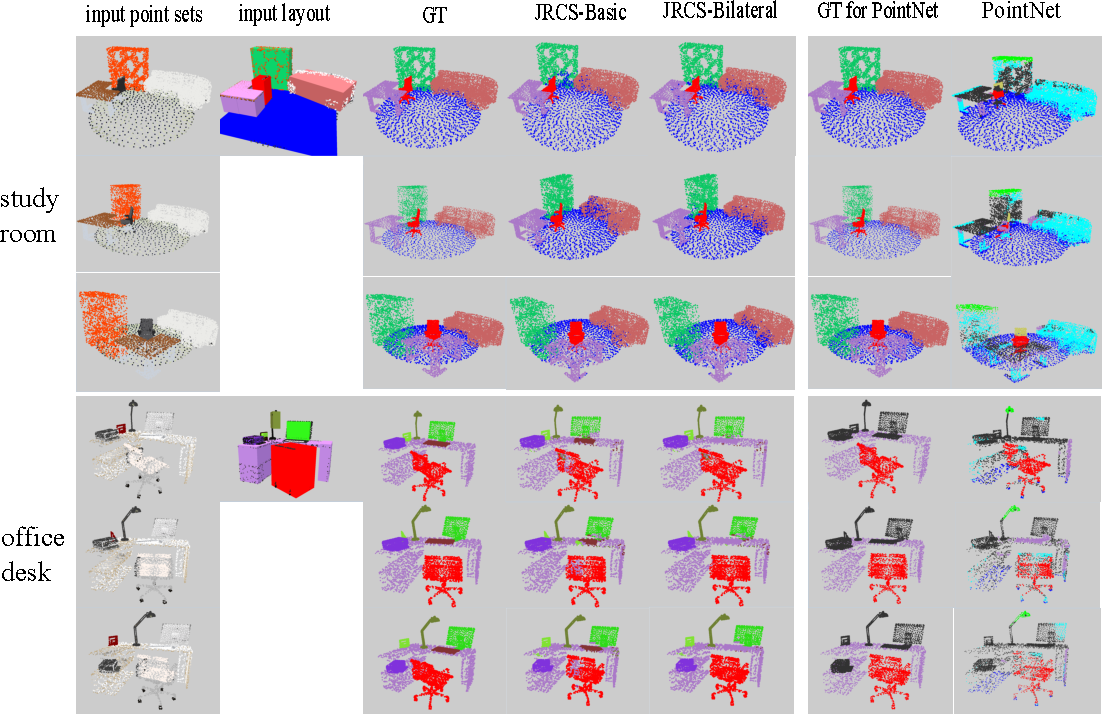
\includegraphics[width=\linewidth]{images/exp/exp_seg}
	\caption{\label{fig:seg} Segmentation evaluations on two groups of synthetic data (study room and office desk). Three examples of point set from each group are shown.}
\end{figure}
%
From the perspective of co-segmentation, we quantitatively evaluate our algorithm on two group of synthetic data of indoor scenes. 
%
To estimate the power of the proposed algorithm, the interaction of placing boxes is only performed at one point set. No further interaction is required. 
% we only input layout for one point set in each group for initialization and do not add further interaction.
%
For numerical estimation, we calculate the intersection over union (IOU) scores for the inducing segmentation against the ground-truth segmentation.
% 
We compare our results with the state of art semantic segmentation method, PointNet~\cite{qi2016pointnet}, which trains a network using a large-scale database. 
%
Table~\ref{tab:seg} shows the numeric result and Figure~\ref{fig:seg} shows visual result of three input point set including the one that is equiped with input layout.
For the object class that is not annotated in the training data, PointNet~\cite{qi2016pointnet} treats it as a special class of "clutter". This is why we have different ground truth for our method and PointNet. As shown in Figure~\ref{fig:seg}, we have "GT" as groundtruth used to evaluate our method and "GT for PointNet" as groundtruth used to evaluate PointNet. 
%
Comparing our method to PointNet is not an exact fair comparison in following aspects:
\begin{enumerate}
\item Our method allows user interaction and PointNet is fully automatic in the test phase.
\item Our synthetic data is quite different from the data in Stanford 3D semantic parsing dataset\cite{semsegdataset} which is used to train the semantic segmentation network of PointNet.
\item Our method outputs object-level segmentation without semantic label, while PointNet outputs semantic labels.  
\end{enumerate}
However, by comparison we can see that the generalization ability of current learning based point set segmentation method is still far from enough to be used as tool to prepare data and build dataset. Semantic segmentation method is limited to certain set of object classes (13 classes for PointNet) and cannot be used to carry on our task. 
\subsection{Evaluation for Joint Registration on Synthetic Data}
From the perspective of joint registration, we first evaluate the result by transferring the point cloud of objects to each input point set based on result $\{\phi_{mn}\}$ and calculating the average distance from a point to its true correspondent point for each input point set.
We use this average distance as fitness error to evaluate the registration quality respect to each input set.

\begin{table}
	\centering
	\caption{Registration errors of the three groups of synthetic data in Figure~\ref{fig:seg}. The errors are measured in meter.}
	\begin{tabular}{c | c c c}
		Method@Dataset&Maximum&Median&Minimum\\
		\hline 
		Basic@Study Room&0.441&0.085&0.027\\
		Bilateral@Study Room&0.139&0.052&1.31e-05\\
	    Basic@Office Desk&0.309&0.0408&5.82e-03\\
		Bilateral@Office Desk&0.222&0.0574&8.33e-03\\
	\end{tabular}
	\label{tab:regerror}
\end{table}
\begin{figure}[htb]
	\centering
	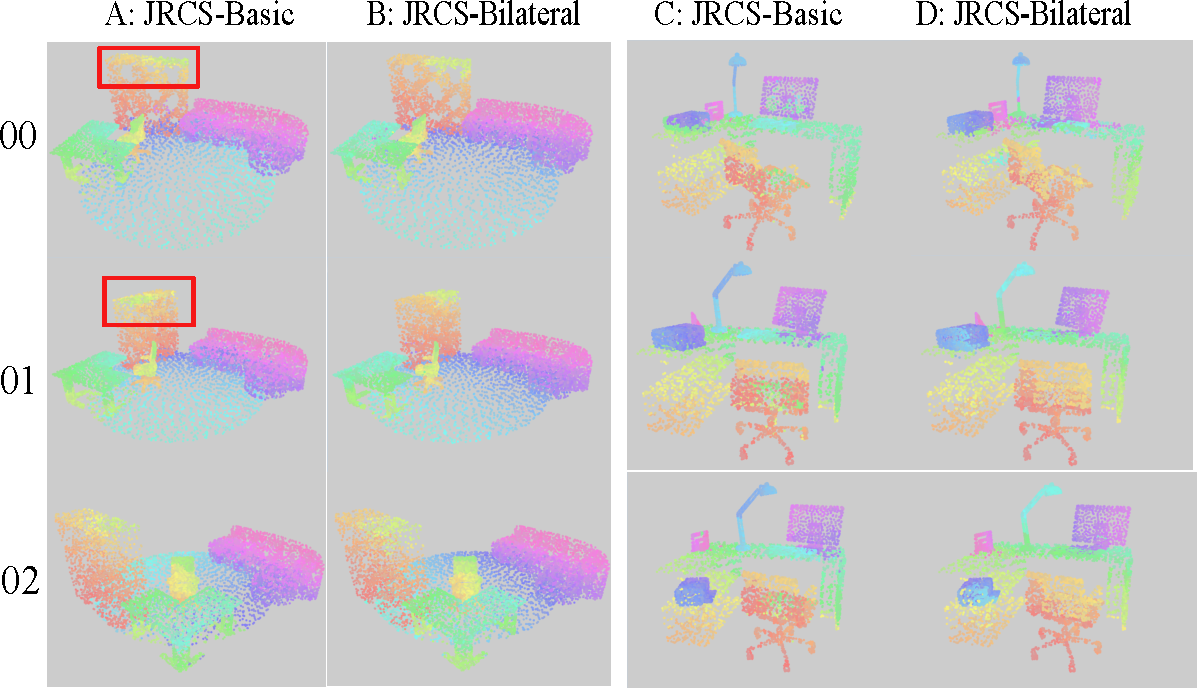
\includegraphics[width=\linewidth]{images/exp/exp_reg}
<<<<<<< HEAD
	\caption{This figure shows some visual examples of joint registration.  The result  is illustrated by color-coding the point-wise correspondences. }
=======
	\caption{Joint registration results on two scenes using two variants of our method. Point-wise correspondences are color-coded.}
>>>>>>> f3b7495718a303c1bdafa2280072981b6697e028
	\label{fig:reg_colorcode}
\end{figure}
Table~\ref{tab:regerror} shows the result of this evaluation. In Table~\ref{tab:regerror} the Maximum, Median and Minimum of the fitness error across input sets are reported.
%
%For this evaluation we want to discuss that:\\
We find that even the input set with high IOU scores in segmentation can result in high fitness error. We believe this is due to the symmetric and near-symmetric objects in the scene. For symmetric objects, even the registration is correct the distance from a point to its true correspondent point can be high, since the rotation in registration result can be different from the one we use to generate this synthetic data. For near-symmetric objects, the registration often gets stuck in a local optimal and results in a high IOU score but a high fitness error. 

Therefore, we show some example of visual result for joint registration in Figure~\ref{fig:reg_colorcode}. By comparing Figure~\ref{fig:reg_colorcode}"A01" and Figure~\ref{fig:reg_colorcode}"A02", we can see that the registration of the round carpet is correct but due to its symmetry its point-wise correspondences are not the same with identity transformation.
By comparing Figure~\ref{fig:reg_colorcode}"A00" and Figure~\ref{fig:reg_colorcode}"A01", (the parts that are highlighted by red rectangle) we can see that registration of the shelf is not correct and it is stucked at a local minimum that maps left part to right part.

We then compare our method (JRCS-Basic) with \cite{Evangelidis2014}(JRMPC) on the synthetic point sets released by \cite{Evangelidis2014}. These data contains four point sets of Stanford Bunny with different noise and outliers. From the experiment result shown in Table~\ref{tab:reg} and Figure~\ref{fig:reg}, we can see that when dealing with one object, our method have similar result with \cite{Evangelidis2014}.

\begin{table}
	\centering
<<<<<<< HEAD
	\caption{This table shows the RMSE of joint registration on 4 point sets of Stanford Bunny. JRMPC is the method of \cite{Evangelidis2014}. JRCS-Basic is our basic formulation}
	\begin{tabular}{c c c c}
		Point Sets& View 2 & View 3 & View 4 \\
		\hline
		JRMPC & 0.1604 & 0.1719 & 0.1838\\   
=======
	\caption{RMSE of joint registration on 4 point sets of Stanford Bunny by two methods.}
	\begin{tabular}{c c c c}
		Point Sets& View 2 & View 3 & View 4 \\
		\hline
		JRMPC~\cite{Evangelidis2014} & 0.1604 & 0.1719 & 0.1838\\   
>>>>>>> f3b7495718a303c1bdafa2280072981b6697e028
		JRCS-Basic & 0.0822 &  0.1570  & 0.2301\\
	\end{tabular}
	\label{tab:reg}
\end{table}
\begin{figure}[htb]
	\centering
	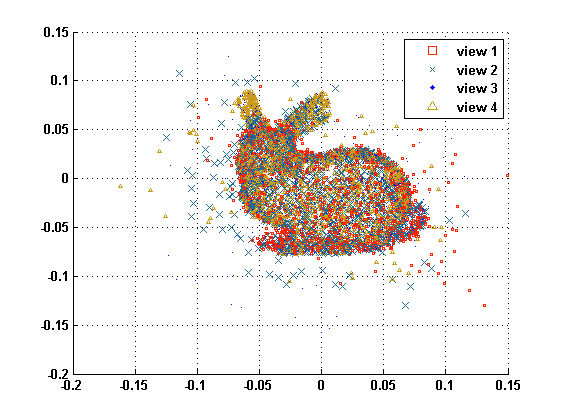
\includegraphics[width=0.4\linewidth]{images/JRMPC.png}
	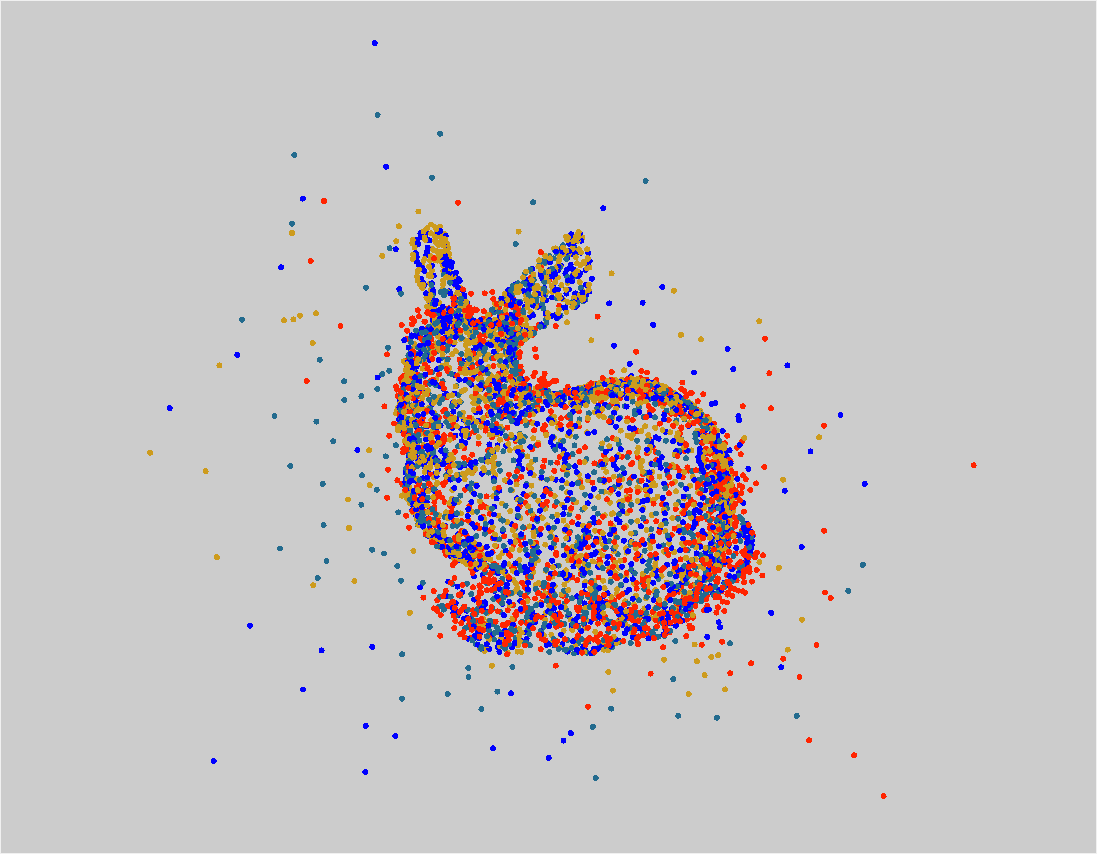
\includegraphics[width=0.4\linewidth]{images/JRCSReg.png}
<<<<<<< HEAD
	\caption{This figure shows the visual result of joint registration on 4 point sets of Stanford Bunny by JRMPC (\cite{Evangelidis2014} at left) and JRCS-Basic (our basic formulation at right)}
=======
	\caption{Joint registration results on 4 point sets of Stanford Bunny by JRMPC~\cite{Evangelidis2014} (left) and our JRCS-Basic (right).}
>>>>>>> f3b7495718a303c1bdafa2280072981b6697e028
	\label{fig:reg}
\end{figure}

\subsection{Investigation on Interaction}
\label{subsec:interact}

For parameter initialization and object shape constraint, we only need the user to input layout (boxes) in one of the input point sets. However, our algorithm sometimes gets stuck at local minimum on handling non-local motion of objects. In such challenging cases, we require more user input to further guide the optimization. In this subsection, we show an example of such challenging case and investigate on the amount of interaction that is needed to improve the result. Figure~\ref{fig:interact_number} shows how the IOU score increases along with the amount of interaction. In this experiment, we use JRCS-Basic. From this experiment,  We can see this from Figure~\ref{fig:interact_number}, the curve of Minimum IOU is not monotonically increasing with the amount of manual input, which means more interaction does not guarantee improvement of the segmentation results in all point sets.  When the initial correspondences in most point sets are far from correct our method loses its ability to transfer the information among different point sets. The further interaction only improves the segmentation in the point set which the user adds layout into and barely improves the segmentation in other point sets.
From Figure~\ref{fig:interact_vis}, we can see that actually quite a lot more interaction is needed for the overall segmentation result to be visually satisfying.
 
\begin{figure}
	\centering
	\includegraphics[width=\linewidth]{images/interact/IOU.png}
<<<<<<< HEAD
	\caption{This figure shows an example of how the amount of interaction affect the IOU score of co-segmentation, the X axis is ratio: $x=\frac{Input~Box~Number}{Total~Object~Number}$. $x=1.0$ means that the user input one box for each object in all point sets}
=======
	\caption{IOU scores of co-segmentation results based on different amount of user interaction. The $X$ axis is the ratio: $x=\frac{Input~Box~Number}{Total~Object~Number}$. $x=1.0$ means that the user places one box for each object in all point sets.}
>>>>>>> f3b7495718a303c1bdafa2280072981b6697e028
	\label{fig:interact_number}
\end{figure}

\begin{figure}
	\centering
	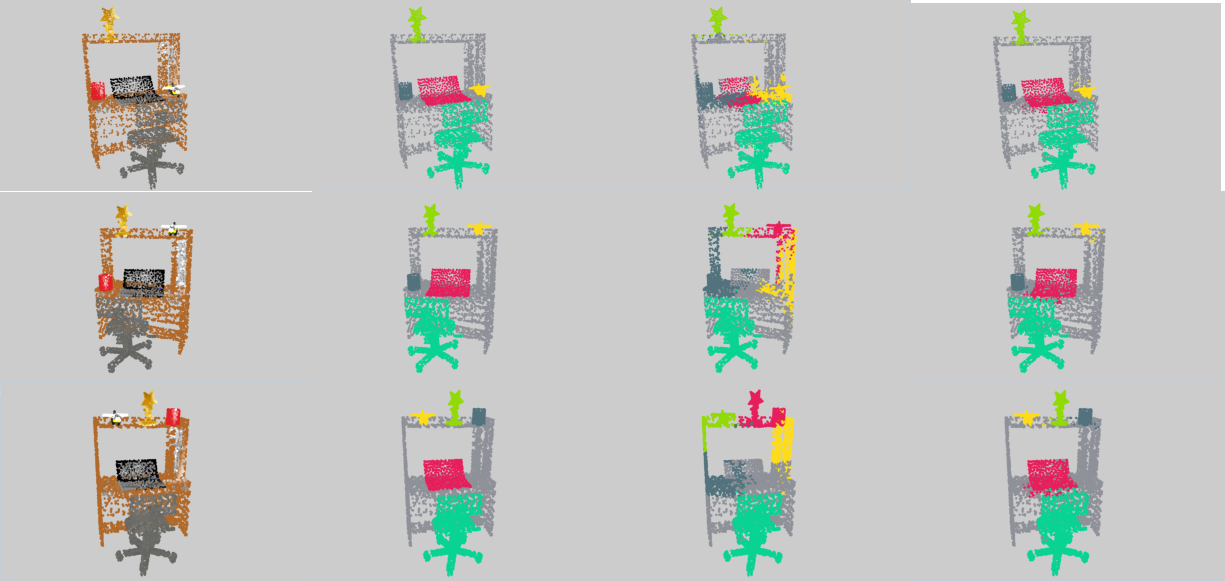
\includegraphics[width=\linewidth]{images/interact/interact}
<<<<<<< HEAD
	\caption{This figure shows 3 out of 16 point sets as examples for experiment on amount of interaction. The column A shows the input point sets, the column B shows the groundtruth segmentation. The column C shows the visual result when 1 point set is equipped with manual input layout. The column D shows the visual result when 11 out of 16 point sets are equipped with manual input layout.
=======
	\caption{Given the same input point sets, more accurate segmentation results can be obtained with more interaction. From left to right: 3 out of 16 input point sets, the ground-truth segmentation, our result when only one point set is equipped with manual input layout, and our result when 11 out of 16 point sets are equipped with manual input layout.
>>>>>>> f3b7495718a303c1bdafa2280072981b6697e028
	}
	\label{fig:interact_vis}
\end{figure}

\subsection{Investigation on Influence of Point Incompleteness}
\label{sec:exp-incompleteness}
In previous evaluation on synthetic data, we use data that the objects are completely covered by the sampled points. 
%
In this subsection, we investigate how the point set incompleteness affect the result of our algorithm. 
%To do this, we pick a group of point sets that can converge well ( IOU $> 99\%$ for each point set ) when the point sets are complete. 
%
To test this, we pick a group of point sets, and gradually remove certain percentage ( $0\%-30\%$ ) of points from each point set. In order to simulate the point incompleteness caused by occlusion using a simple method, we generate the incomplete point sets with incompleteness of $p\%$ as follows:
\begin{enumerate}
	\item We randomly pick one point from each complete point set. 
	\item For one point set, sort all points ascending according to their euclidean distance to the picked point.  
	\item Remove the first $p\%$ points from the point set to generate a point set with incompleteness of $p\%$.
\end{enumerate}
% 
Figure~\ref{fig:incompleteness} shows how the IOU score is affected with the increasing point set incompleteness in this experiment. 
Figure~\ref{fig:incompleteness2} shows some example of visual result in this experiment. The results of $p=\{0.0,14.0,30.0\}$ are shown. In Figure~\ref{fig:incompleteness2}(A09-E09), we can see that for some object in the scene half of the points are already removed. From the result we can see that even with serious incompleteness on some of the objects our algorithm converge to a relative good result.

\begin{figure}
	\centering
	\includegraphics[width=\linewidth]{images/incompleteness/IOU.png}
<<<<<<< HEAD
	\caption{This figure shows how the data incompleteness affect the IOU score of co-segmentation. The data used in this experiment is partially shown in Figure~\ref{fig:incompleteness2}.}
=======
	\caption{IOU scores of co-segmentation with different data incompleteness. The used data is partially shown in Figure~\ref{fig:incompleteness2}. }
>>>>>>> f3b7495718a303c1bdafa2280072981b6697e028
	\label{fig:incompleteness}
\end{figure}
\begin{figure}
	\centering
	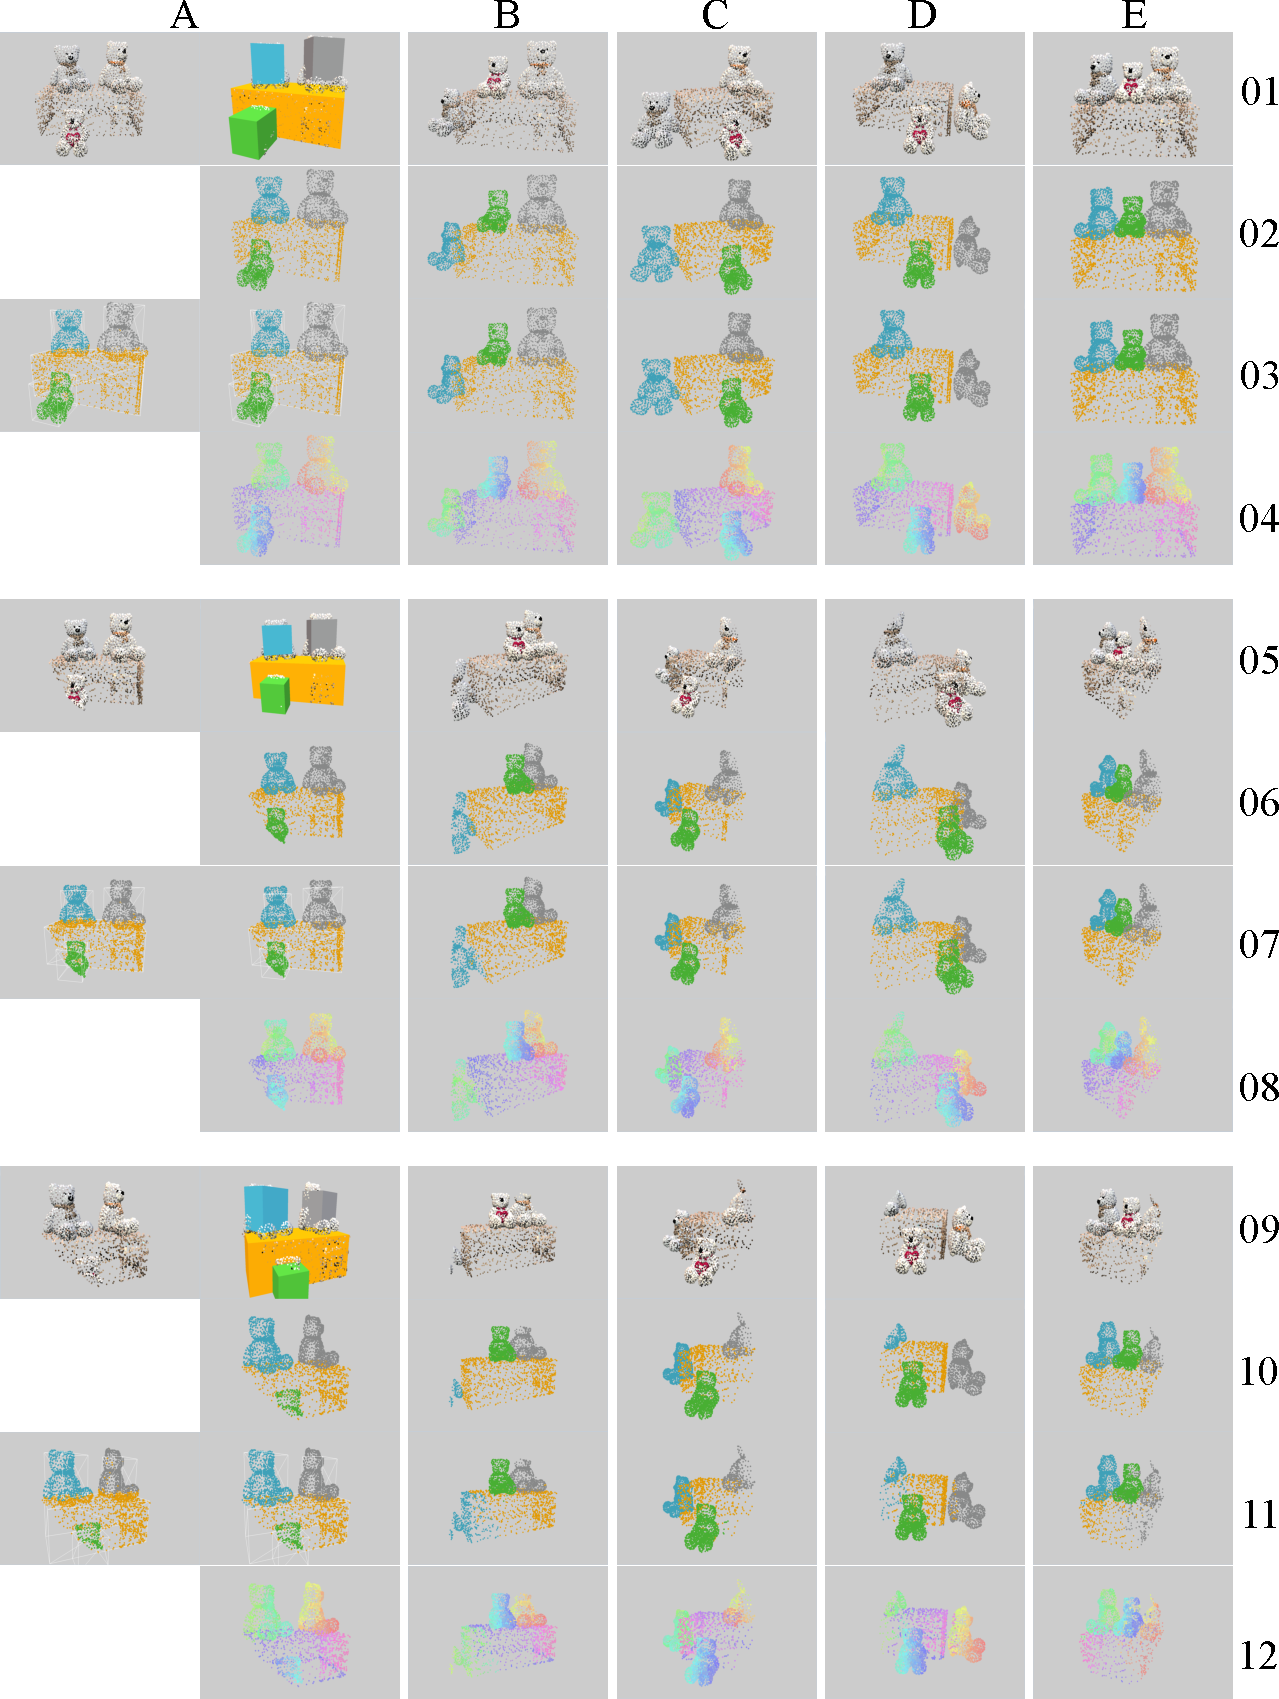
\includegraphics[width=\linewidth]{images/incompleteness/visual}
	\caption{Experiments on data incompleteness. This figure shows results at 3 different level of incompleteness which are $0.0\%$ at row 01-04, $14\%$ at row 05-08 and $30\%$ at row 09-12. Each column shows the information of the same point set. Rows 01, 05, 09 show the inputs. 
	Column A shows one point set and the manual input for initialization. 
	The initial segmentation and final segmentation of this point set are shown in column A as well.
	Row 02,06,10 are ground-truth of segmentation. Row 03,07,10 are our segmentation results. 
	Row 04,08,12 shows the point-wise correspondences of joint registration by color-coding.}
	\label{fig:incompleteness2}
\end{figure}
\subsection{Test On Real Data}
To capture real data we employ the voxel hashing method~\cite{VXH} and use plane fitting to remove walls and floors. 
%
We then transfer the meshes into point sets using a Poisson sampling process~\cite{PossionSampling}.
%
Figure~\ref{fig:challenge} shows a scanned point set. We can see that, there are noised and blurred color, shape distortion, partial scanning and outliers in real data.
%
Figure~\ref{fig:realdata} shows the segmentation and registration results on a group of scanned point sets We uses JRCS-Bilateral in this test and Figure~\ref{fig:realdata}(d) shows the only point set that is equipped with layout in this test.
From Figure~\ref{fig:realdata}(e), we can see that all input point sets are partitioned into objects. In Figure~\ref{fig:realdata}(g), we align the point sets all together respecting to each of the objects. There are four objects in the scene, so there are four different aligned result in Figure~\ref{fig:realdata}(g). The light blue rectangle highlights the object that is used to align the point sets. We can verify that the objects from each input set are aligned together by the result transformation.
\begin{figure}
	\centering
	\includegraphics[width=\linewidth]{images/challenge/challenge}
	\caption{\label{fig:challenge}Common challenges in scanned data.}
\end{figure}
\begin{figure*}
	\centering
	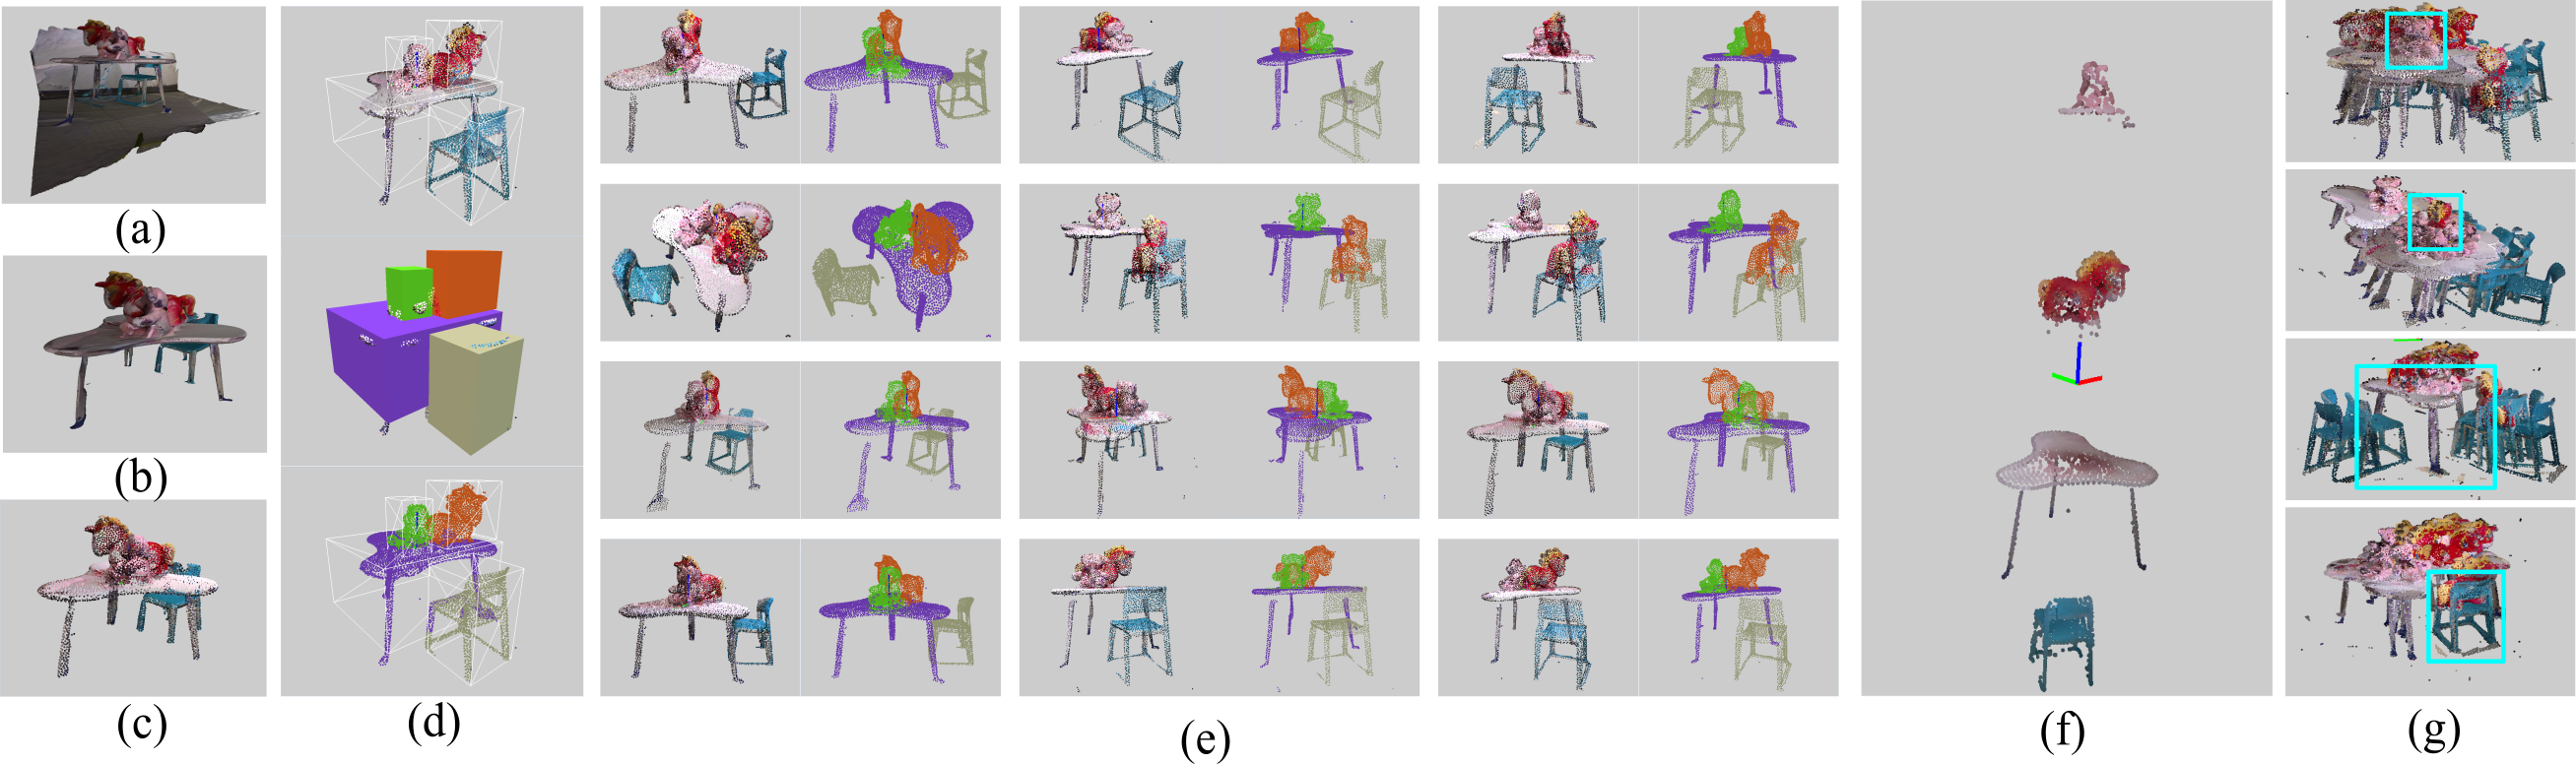
\includegraphics[width=\linewidth]{images/realdata/realdata}
	\caption{\label{fig:realdata} Segmentation and registration on real data. (a) Scanned mesh using method in \cite{VXH}. (b) Remove walls and floors by plane fitting. (c) Sampled point set using \cite{PossionSampling}. (d) With roughly placed boxes on only one point set, the points are initially segmented in this one point set. Note that parts of the chair legs are segmented to the table due to the rough box placement by users. (e) Pairs of input point sets and corresponding segmentation results. (f) The final Gaussian centroids for the five objects in the scene. (g) Verification of the registration result by aligning all point sets with respect to each object. The light blue rectangle highlights the object that is aligned together. Except the aligned object, the other objects are placed quite messy since they came from different point sets and have different arrangement relative to the aligned object. %\cxj{Again, i think (g) is really messy and confusing...}  
	}
\end{figure*} 
\subsection{Conclusions}
For the challenging problem of point set joint registration and co-segmentation, we come up with a formulation simultaneously modeling the two entangled sub-problems. For the difficult initialization and optimization of this formulation, we provide a strategy that lean on a few manual inputs. In the evaluation, our algorithm have some success on both synthetic and real data.
The practical issue holding us back is the time performance of our current implementation, which prevents us from going over more initialization and optimization strategies. For a group of 11 point sets with about 9K points in each point set, our current implementation will take about 110 minutes to run 100 iteration.  
With a parallelized implementation, we can probably explore more potentials of our algorithm and try it on a scene of a larger scale by drawing experience from \cite{GOGMA} and \cite{AGM}. 